\subsection{RQ4: Test smells and revisions}
The previous analysis shows that revisions to test methods are not necessarily driven solely by changes in the production methods they exercise. Test methods may also evolve because of internal maintainability issues. Test smells provide a useful lens for examining this possibility, as they capture potentially problematic characteristics of test code~\cite{bavota2015test,Spadini:2018,panichella2022test}. Prior work has shown that test smells are most often introduced in the initial version of a test method~\cite{tufano2016empirical}. Therefore, this section investigates whether the presence of test smells in the first version of a test method is associated with a high number of future revisions.

\subsubsection{Approach}
For smell detections, \emph{JNose}~\cite{virginio2020jnose} was used. Using rule-based detectors derived from established test-smell definitions and detection rules from prior work~\cite{tufano2016empirical,garousi2018smells}, \emph{JNose} detects different types of test smells and provides method-level smell locations, making it appropriate for this analysis. To understand the association of test smells with method evolution, the test methods are divided into three groups and labeled for easy reference for subsequent analysis.
\begin{itemize}
    \item \textbf{NTR}: These are methods that were not revised more than their corresponding production methods (normal test revision).
    \item \textbf{MTR}: These methods were revised more than their production methods (more test revisions).
    \item \textbf{HTR}: A subset of \emph{MTR}, these methods were revised at least five more times than their production methods (high test revisions).
\end{itemize}

A test method may exercise multiple production methods and, as a result, may
receive different group assignments depending on which linked production method
is used. To reduce ambiguity, such methods were filtered out for this RQ. Also, to ensure
sufficient project-level coverage, projects for which the strategy establishes at least 30 links were included. After applying this threshold, the resulting sample includes 71,231 \emph{NTR} methods from 90 projects, 23,494 \emph{MTR} methods from 88 projects, and 3,274 HTR methods from 74 projects.

The following metrics were used for comparing these three groups of methods.
\begin{itemize}
    \item \textbf{Percent (\%):} For each individual smell, its prevalence was calculated in the three groups of methods. The difference in percent (\textbf{$\Delta$ pp}) was also calculated.
    \item \textbf{Odds ratio (OR):} Suppose the odds ratio is calculated by using \emph{NTR} and \emph{HTR} groups. Let $a$ be the number of HTR methods with a smell, $b$ the
number of HTR methods without the smell, $c$ the number of NTR methods with the
smell, and $d$ the number of NTR methods without the smell. The odds ratio is
computed as $\mathrm{OR} = (a/b)/(c/d) = ad/bc$, so values above one indicate
that the smell is more prevalent among HTR methods. The conditional
maximum likelihood estimate of the odds ratio and its exact 95\% confidence
interval are reported.
\item  \textbf{Fisher's
exact tests ($p_{BH}$)~\cite{fisher1922interpretation}:} Two-sided Fisher's
exact tests were also used because the group sizes are unequal and several smells are rare. The
Benjamini--Hochberg~\cite{benjamini1995controlling} procedure was also applied across the individual-smell comparisons to
control the false discovery rate at 0.05.
\item \textbf{Mantel-Haenszel (\textbf{MH OR}} and \textbf{MH $p_{BH}$})~\cite{mantel1959statistical}: Projects may differ in their testing practices and baseline smell prevalence.
As a sensitivity analysis, a Mantel-Haenszel odds
ratio was additionally estimated for each smell while treating projects as strata, and the same
multiple-comparison correction.
% \textcolor{red}{Agreement between the pooled and
% project-stratified results indicates that an association is not explained
% solely by differences among projects.}


\end{itemize}
% , and the odds ratio
% with a 95\% confidence interval. For each smell, we form a $2 \times 2$
% contingency table.  We use two-sided Fisher's
% exact tests because the group sizes are unequal and several smells are rare. We apply the
% Benjamini--Hochberg procedure across the individual-smell comparisons to
% control the false discovery rate at 0.05.

% Projects may differ in their testing practices and baseline smell prevalence.
% As a sensitivity analysis, we additionally estimate a Mantel--Haenszel odds
% ratio for each smell while treating projects as strata, and apply the same
% multiple-comparison correction.  Agreement between the pooled and
% project-stratified results indicates that an association is not explained
% solely by differences among projects.

% We also visualize the distribution of test-method revision counts for NTR and
% HTR methods using boxplots. In addition, we summarize the count-based
% comparison in prose rather than displaying the full generated table. To examine
% whether the observed smell--revision associations are sensitive to method size,
% we also repeat the top-five-smell comparison within LOC-based control groups.
% Following the size-control grouping used in prior test-smell
% work~\cite{Spadini:2018}, we classify test methods as small, medium, or large
% based on the LOC of the introduced version analyzed by JNose. Specifically,
% small methods have fewer than $30$ LOC, medium methods have $30$--$60$ LOC, and
% large methods have more than $60$ LOC. These fixed ranges allow us to compare
% HTR--NTR and MTR--NTR differences within methods of comparable size.

\subsubsection{Result}
% \begin{figure}[ht]
%     \centering
%     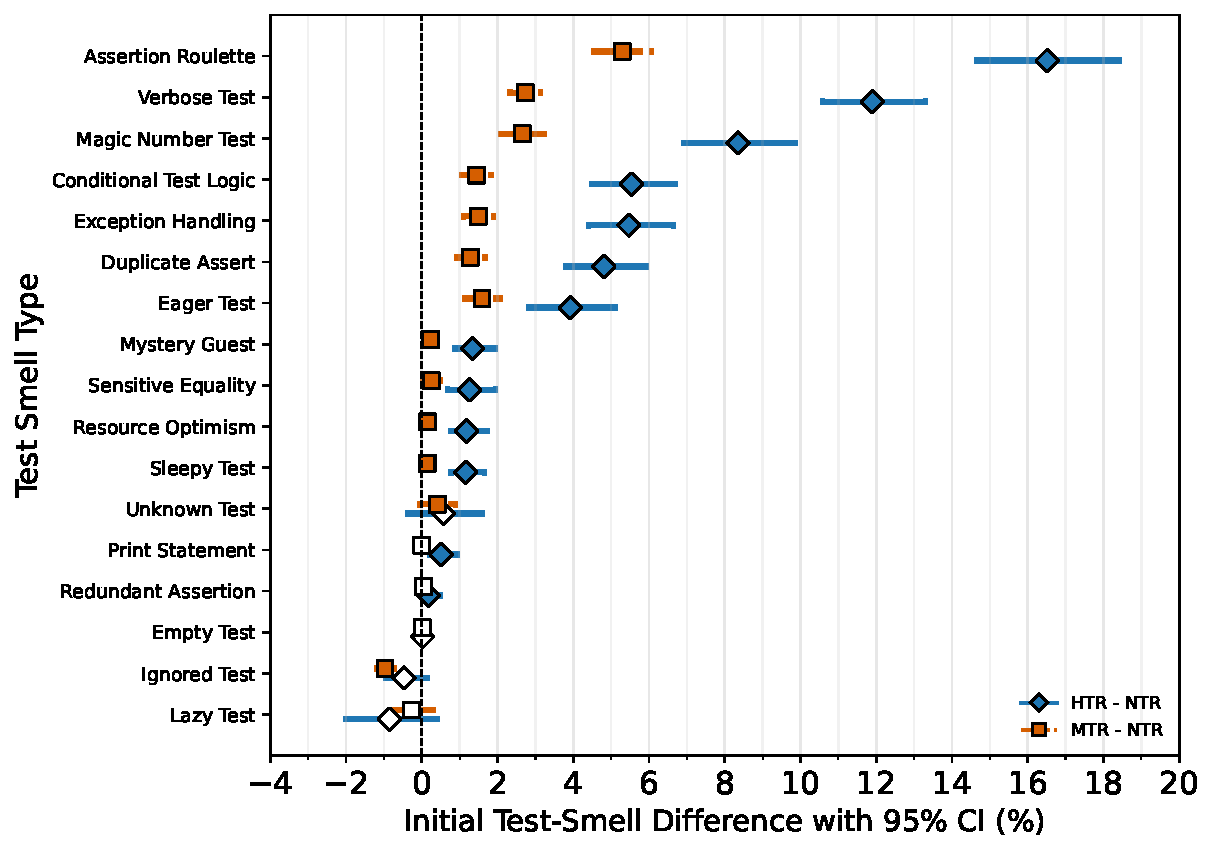
\includegraphics[width=\linewidth]{figure/t2p-test-smell-effectplot--historyFinder--omc--nc--jnose--ch_diff.pdf}
% \caption{Initial test-smell prevalence differences for HTR--NTR and MTR--NTR comparisons. The x-axis reports differences in percentage points; positive values indicate higher smell prevalence in HTR or MTR than in NTR, respectively. Overall, at least one test smell is more prevalent in HTR than NTR by 20.8 percentage points and in MTR than NTR by 6.3 percentage points. Diamonds with solid intervals denote HTR--NTR, whereas squares with dashed intervals denote MTR--NTR. Filled markers indicate Benjamini--Hochberg-significant smells; open markers indicate non-significant smells. Error bars show 95\% confidence intervals.}
% \label{fig:rq4-test-smell-effect}
% \end{figure}


% \begin{figure}[ht]
%     \centering
%     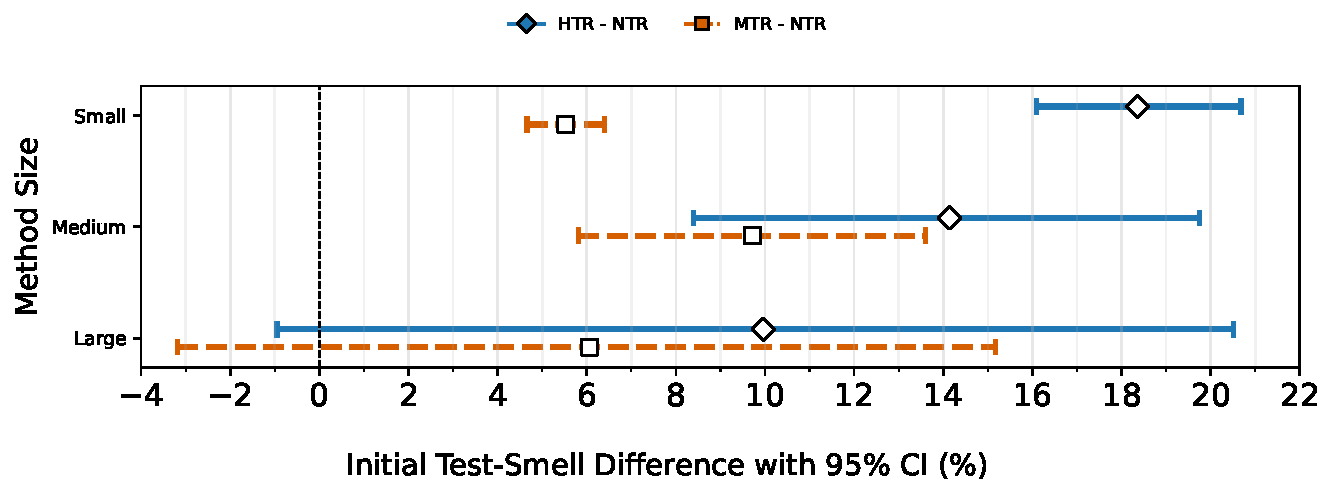
\includegraphics[width=\linewidth, keepaspectratio]{figure/t2p-test-smell-size-control-effectplot--historyFinder--omc--nc--jnose--ch_diff.pdf}
%     \caption{Difference in initial top-five test-smell prevalence by method
%     size. The plot compares HTR--NTR and MTR--NTR within each LOC control
%     group, where TOP5 means that a method contains at least one of Assertion
%     Roulette, Verbose Test, Magic Number Test, Conditional Test Logic, or
%     Exception Handling. Positive values indicate higher prevalence in HTR or
%     MTR than in NTR; intervals show 95\% confidence intervals.
%     The correlation analysis shows a positive association between method size and
% the number of selected top smells. Spearman's correlation is $\rho = 0.34$
% ($p < .001$; medium effect), Kendall's correlation is $\tau = 0.28$
% ($p < .001$; small effect), and Pearson's correlation is $r = 0.36$
% ($p < .001$; medium effect).
% }
%     \label{fig:rq2-test-smell-size-control-effect}
% \end{figure}

% \begin{figure}[ht]
%   \caption{LOC-controlled difference in initial robust-smell prevalence.
%     Each row is a method-size control group. The plotted outcome is whether a
%     method contains at least one smell that is significant in both the pooled and
%     project-adjusted association analyses for the corresponding comparison.
%     Positive values indicate higher prevalence in HTR or MTR than in NTR;
%     intervals show 95\% confidence intervals.}
%     \centering
%     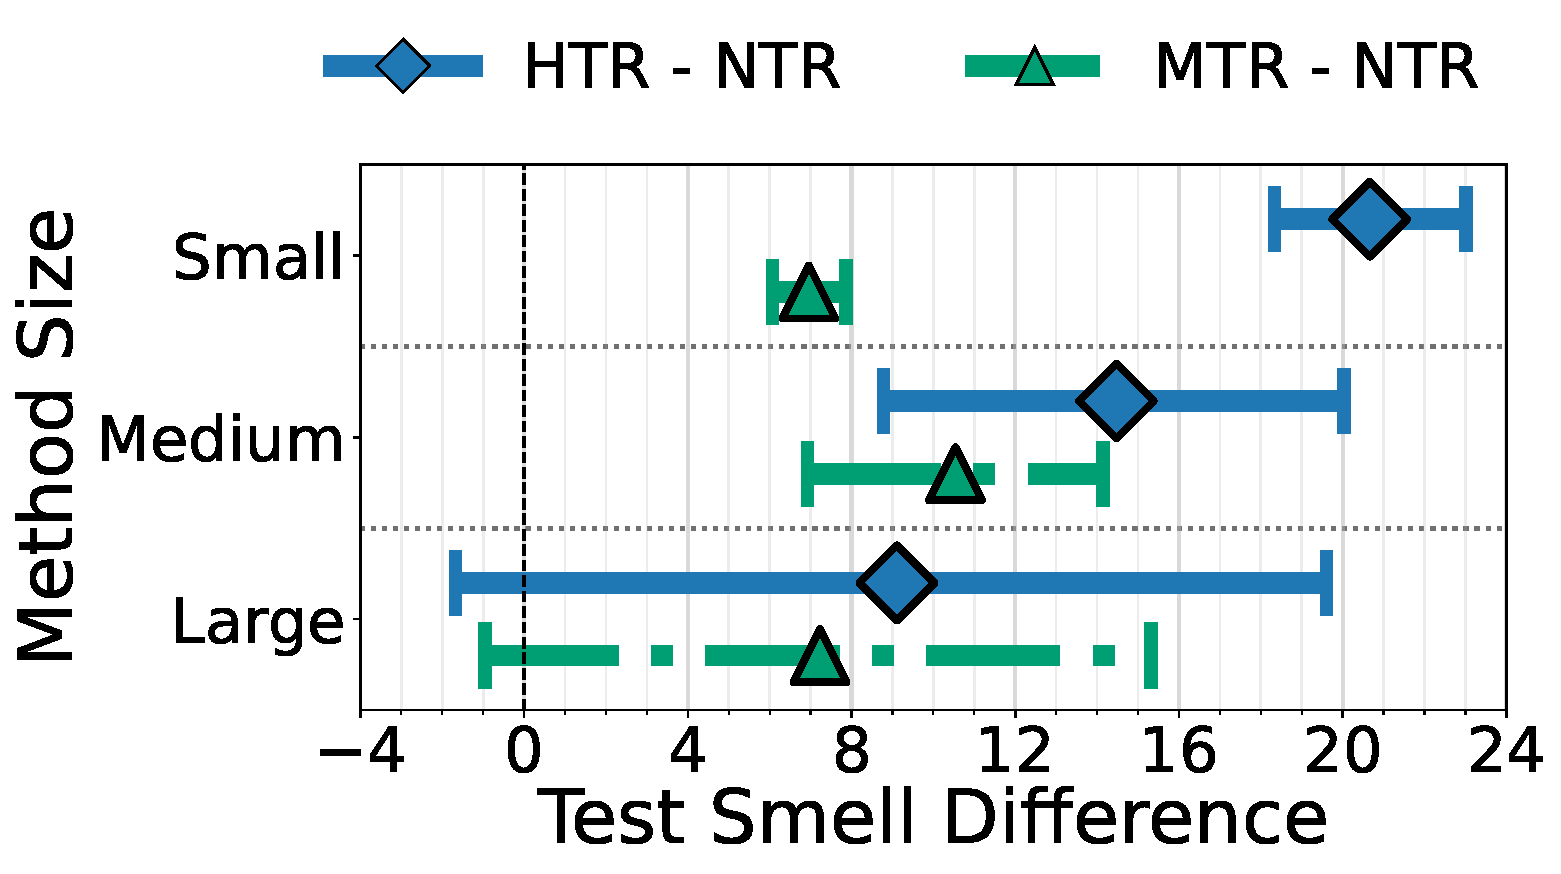
\includegraphics[width=\linewidth]{figure/t2p-test-smell-size-control-effectplot--historyFinder--omc--nc--jnose--ch_diff--HTR-NTR-MTR-NTR}
% \end{figure}
% \begin{figure}[ht]
%  \caption{LOC-controlled odds ratios for initial robust-smell prevalence.
%     Each point estimates the odds that a method in HTR or MTR contains at
%     least one robust-significant smell compared with NTR methods in the same
%     size group. Values above one indicate greater odds in the revision-prone
%     group; intervals show 95\% confidence intervals.}
%     \centering
%     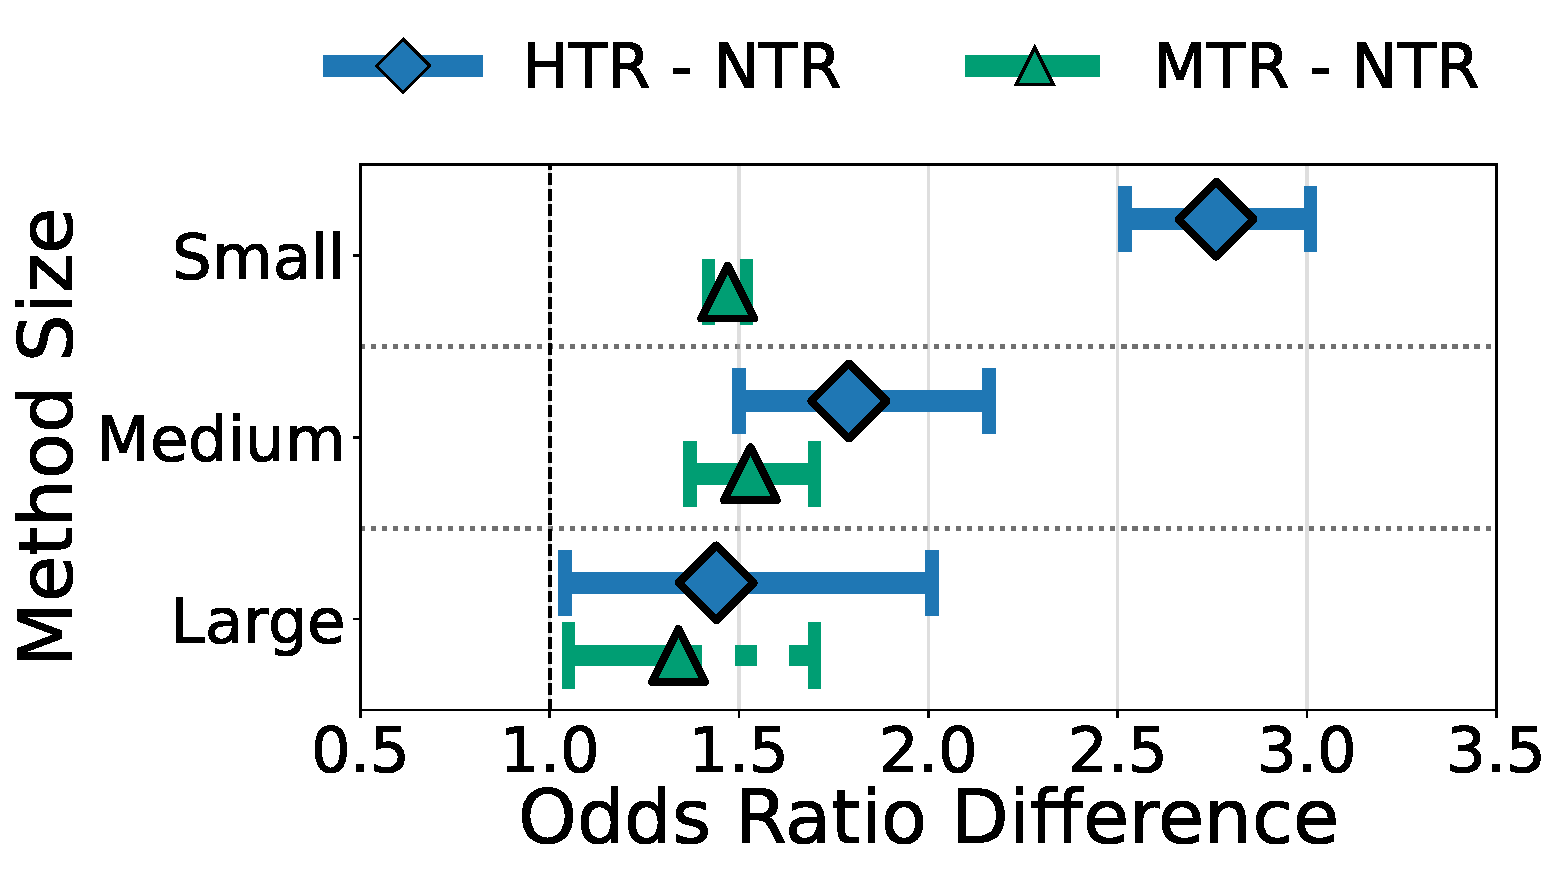
\includegraphics[width=\linewidth]{figure/t2p-test-smell-size-control-odds-ratio-effectplot--historyFinder--omc--nc--jnose--ch_diff--HTR-NTR-MTR-NTR}
% \end{figure}

% \begin{table*}[ht]
% \centering
% \caption{The top part of the table shows results for comparison between the \emph{NTR} and \emph{MTR} methods. For example, \textbf{NTR \%} reports the percent of methods in the \emph{NTR} group with a particular smell. The bottom part shows the comparisons between the \emph{NTR} and \emph{HTR} methods for a few smells. The full table for the bottom part is available (\texttt{/data/rqs/rq4/test-smell-difference.pdf}).}
% %\protect footnotemark}
% \label{tab:rq4-ntr-mtr}

% \small
% \begin{tabular}{lrrrrrrr}
\toprule
\textbf{Test smell} & \textbf{NTR \%} & \textbf{MTR \%} & \textbf{$\Delta$ pp} &
\textbf{OR [95\% CI]} & \textbf{$p_{BH}$} & \textbf{MH OR} & \textbf{MH $p_{BH}$} \\
\midrule
Assertion Roulette & 13.5 & 20.1 & +6.6 & 1.61 [1.55, 1.68] & $<.05$ & 1.48 & $<.05$ \\
Verbose Test & 2.4 & 6.2 & +3.8 & 2.67 [2.49, 2.86] & $<.05$ & 2.30 & $<.05$ \\
Magic Number Test & 7.0 & 10.4 & +3.3 & 1.52 [1.45, 1.60] & $<.05$ & 1.48 & $<.05$ \\
Exception Handling & 3.0 & 4.9 & +1.9 & 1.69 [1.57, 1.82] & $<.05$ & 1.70 & $<.05$ \\
Conditional Test Logic & 2.8 & 4.7 & +1.9 & 1.72 [1.59, 1.85] & $<.05$ & 1.71 & $<.05$ \\
Eager Test & 4.5 & 6.3 & +1.9 & 1.44 [1.36, 1.54] & $<.05$ & 1.51 & $<.05$ \\
Duplicate Assert & 2.8 & 4.5 & +1.7 & 1.64 [1.52, 1.77] & $<.05$ & 1.45 & $<.05$ \\
Unknown Test & 5.2 & 5.6 & +0.4 & 1.09 [1.02, 1.16] & $<.05$ & 0.93 & 0.057 \\
Mystery Guest & 0.5 & 0.9 & +0.4 & 1.73 [1.46, 2.06] & $<.05$ & 1.63 & $<.05$ \\
Sensitive Equality & 1.1 & 1.5 & +0.4 & 1.32 [1.17, 1.50] & $<.05$ & 1.46 & $<.05$ \\
Resource Optimism & 0.4 & 0.7 & +0.3 & 1.71 [1.40, 2.07] & $<.05$ & 1.61 & $<.05$ \\
Sleepy Test & 0.2 & 0.5 & +0.3 & 2.31 [1.78, 2.98] & $<.05$ & 2.76 & $<.05$ \\
Print Statement & 0.3 & 0.4 & +0.1 & 1.19 [0.92, 1.51] & 0.173 & 2.65 & $<.05$ \\
Redundant Assertion & 0.2 & 0.2 & +0.1 & 1.34 [0.97, 1.83] & 0.084 & 1.96 & $<.05$ \\
Empty Test & 0.1 & 0.1 & +0.0 & 1.31 [0.67, 2.45] & 0.420 & 2.03 & 0.072 \\
Lazy Test & 9.2 & 8.9 & -0.3 & 0.96 [0.91, 1.01] & 0.106 & 0.96 & 0.106 \\
Ignored Test & 2.0 & 1.1 & -0.9 & 0.54 [0.47, 0.61] & $<.05$ & 0.40 & $<.05$ \\%\hline\hline\\
\toprule
\textbf{Test smell} & \textbf{NTR \%} & \textbf{HTR \%} & \textbf{$\Delta$ pp} &
\textbf{OR [95\% CI]} & \textbf{$p_{BH}$} & \textbf{MH OR} & \textbf{MH $p_{BH}$} \\
\midrule
Assertion Roulette & 13.5 & 30.0 & +16.5 & 2.75 [2.53, 2.98] & $<.05$ & 2.42 & $<.05$ \\
Verbose Test & 2.5 & 14.3 & +11.9 & 6.66 [5.94, 7.46] & $<.05$ & 5.47 & $<.05$ \\
Exception Handling & 3.0 & 8.4 & +5.5 & 3.01 [2.62, 3.45] & $<.05$ & 3.08 & $<.05$ \\
Conditional Test Logic & 2.8 & 8.3 & +5.5 & 3.15 [2.74, 3.61] & $<.05$ & 2.78 & $<.05$ \\
Duplicate Assert & 2.8 & 7.6 & +4.8 & 2.86 [2.47, 3.29] & $<.05$ & 2.44 & $<.05$ \\
Sleepy Test & 0.2 & 1.4 & +1.2 & 6.97 [4.78, 9.96] & $<.05$ & 9.57 & $<.05$ \\
\bottomrule
\end{tabular}

% \end{table*}


% \begin{figure*}[htbp]
% \centering
% \mbox{
% \subfigure[]{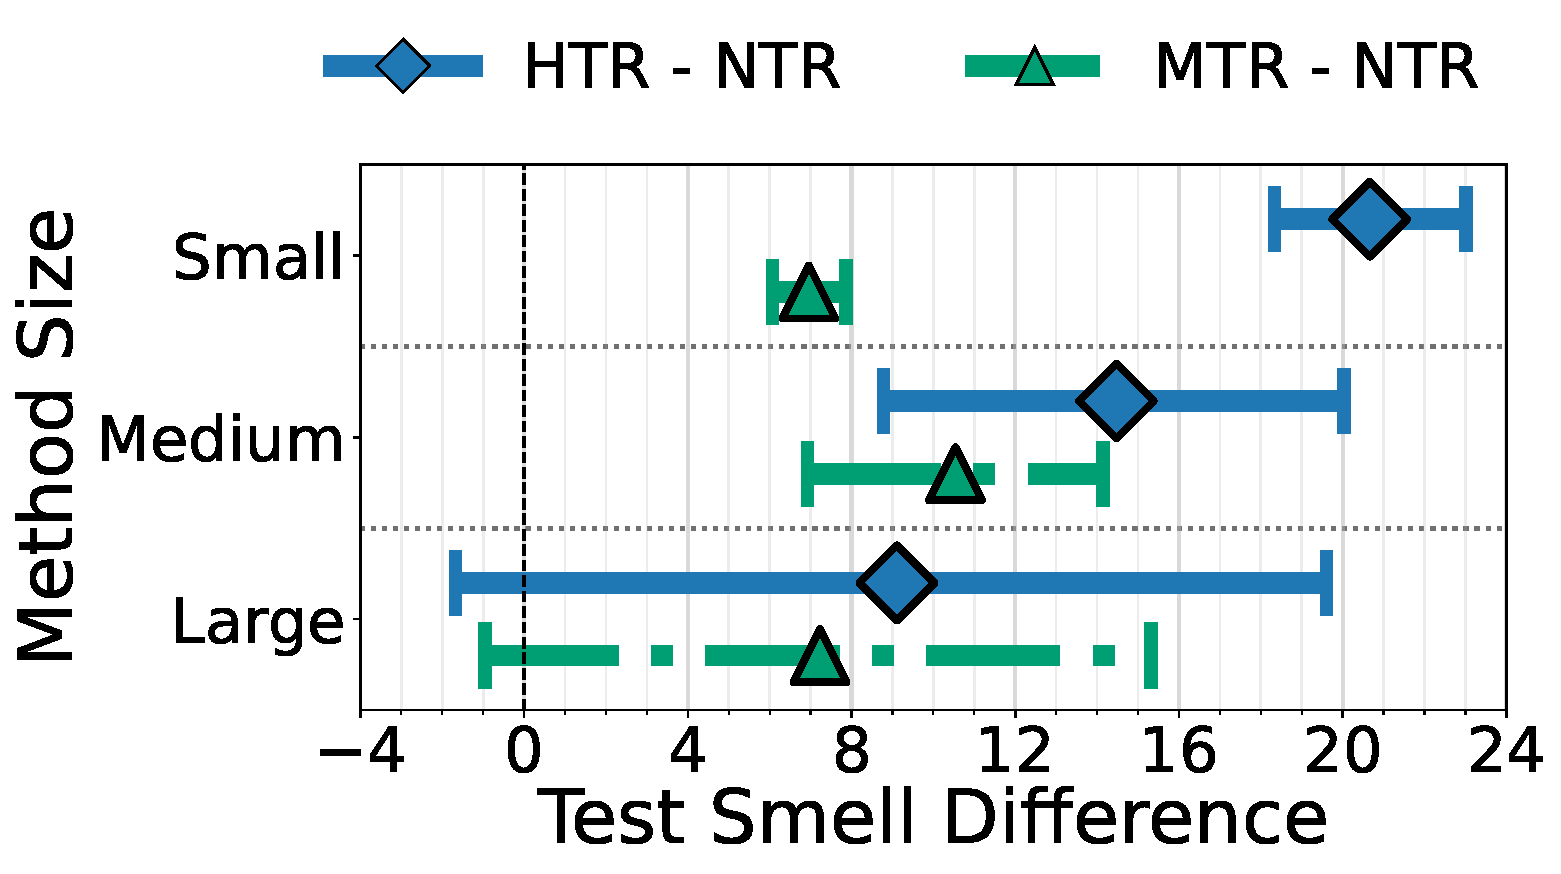
\includegraphics[width=0.38\textwidth,keepaspectratio]{figure/t2p-test-smell-size-control-effectplot--historyFinder--omc--nc--jnose--ch_diff--HTR-NTR-MTR-NTR}}
% \subfigure[]{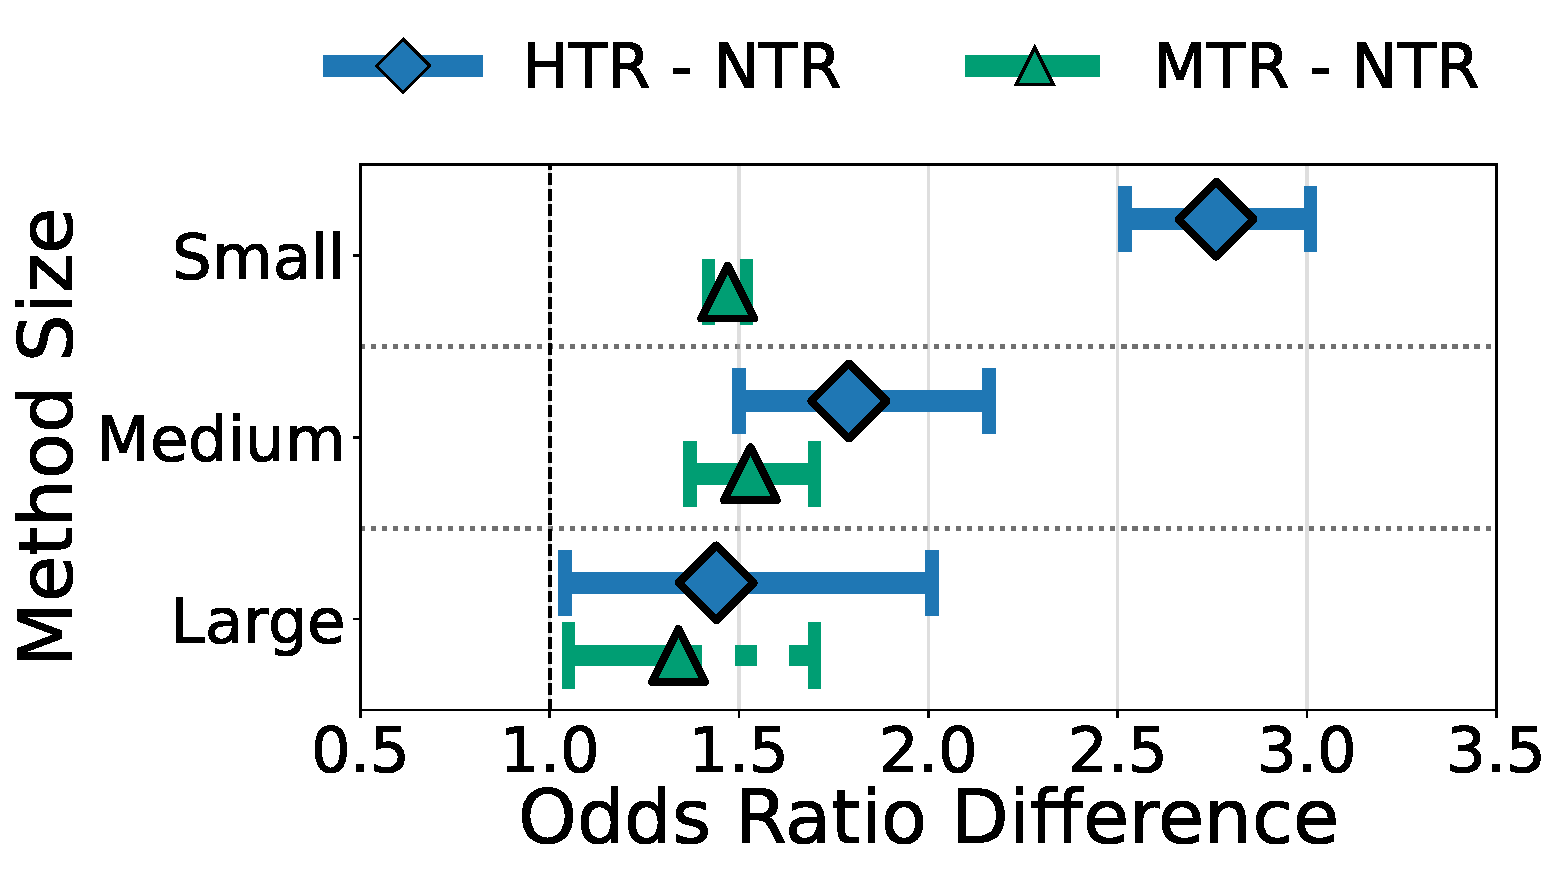
\includegraphics[width=0.38\textwidth,keepaspectratio]{figure/t2p-test-smell-size-control-odds-ratio-effectplot--historyFinder--omc--nc--jnose--ch_diff--HTR-NTR-MTR-NTR}
% }
% }
% \caption{Size-based analysis. Figure (a) shows the difference in percent with 95\% confidence interval, and Figure (b) shows the odds ratio (OR). The comparison is for \emph{MTR} and \emph{NTR} methods, as well as \emph{HTR} and \emph{NTR} methods. The selected 11 types of smells are joined together and considered as one smell.}
% % Figure a label should be Test smell difference, Figure b label should be Odds ratio difference. Both figures are currently unreadable.
% \label{fig:size}
% \end{figure*}


\begin{figure*}[htbp]
\centering

\begin{subfigure}[t]{0.44\textwidth}
    \centering
    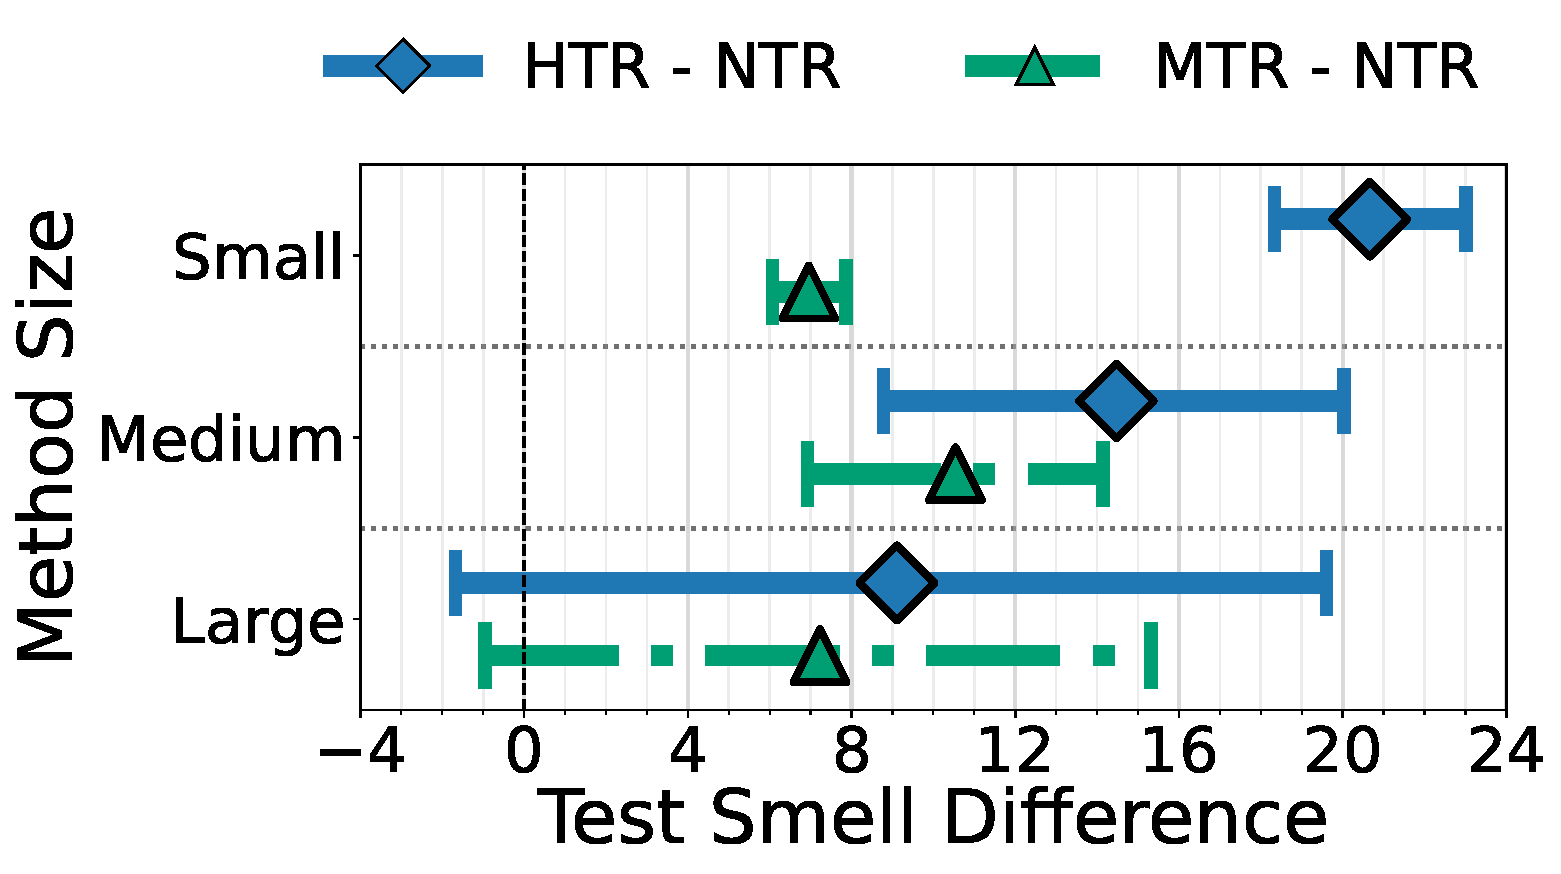
\includegraphics[width=\linewidth,keepaspectratio]{figure/t2p-test-smell-size-control-effectplot--historyFinder--omc--nc--jnose--ch_diff--HTR-NTR-MTR-NTR}
    \caption{}
    \label{fig:size-a}
\end{subfigure}
\hfill
\begin{subfigure}[t]{0.44\textwidth}
    \centering
    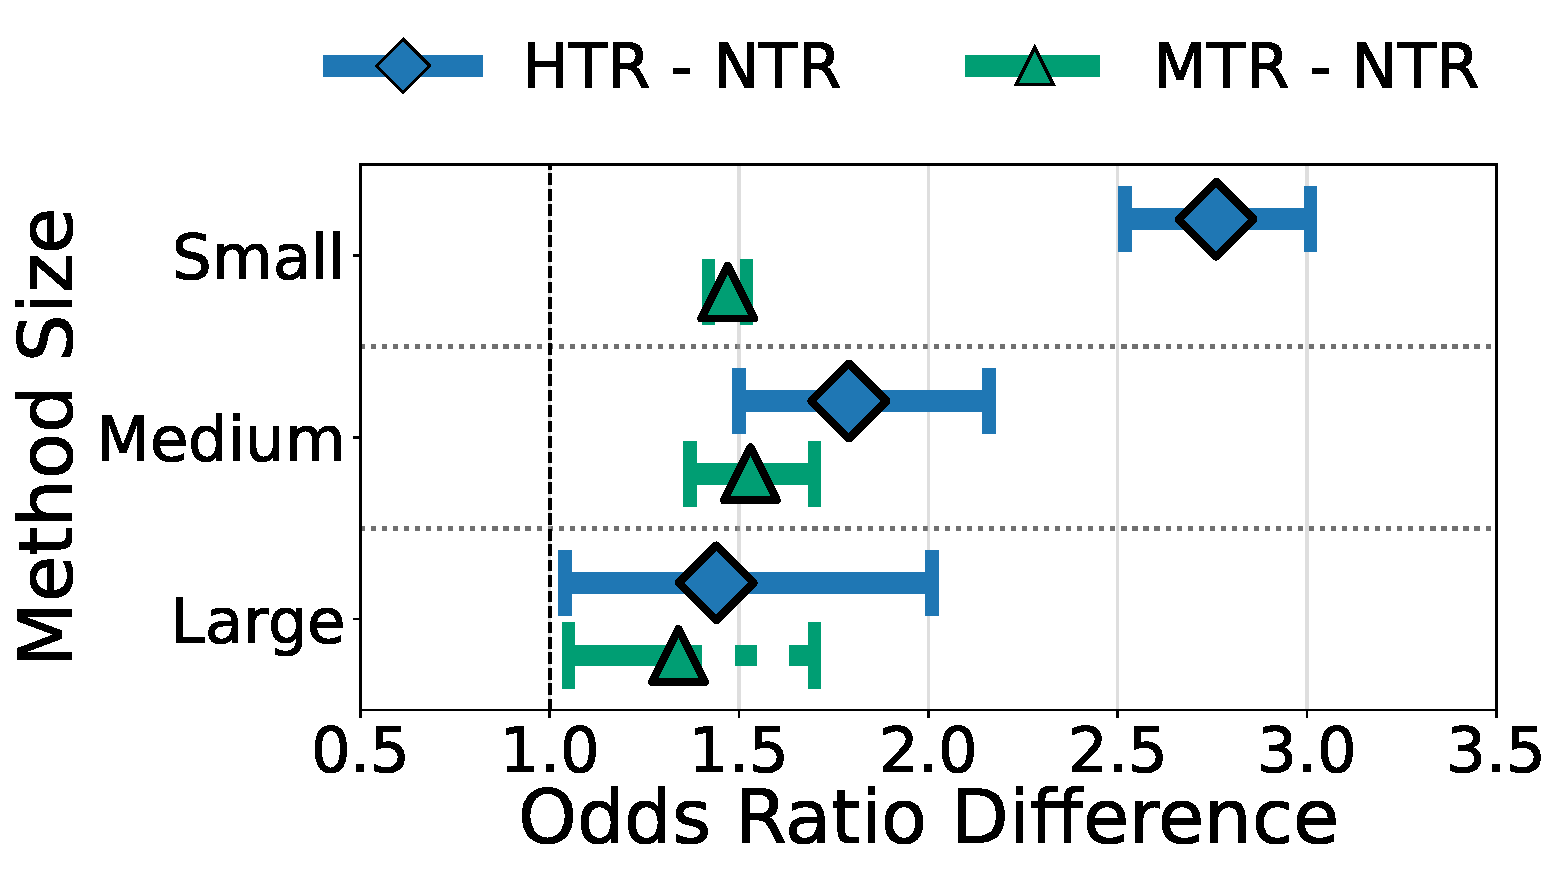
\includegraphics[width=\linewidth,keepaspectratio]{figure/t2p-test-smell-size-control-odds-ratio-effectplot--historyFinder--omc--nc--jnose--ch_diff--HTR-NTR-MTR-NTR}
    \caption{}
    \label{tab:rq4-ntr-mtr}
\end{subfigure}

\caption{Size-based analysis. Figure (a) shows the difference in percent with 95\% confidence interval, and Figure (b) shows the odds ratio (OR). The comparison is for \emph{MTR} and \emph{NTR} methods, as well as \emph{HTR} and \emph{NTR} methods. The selected 11 types of smells are joined together and considered as one smell.}
\label{fig:size}
\end{figure*}



% \begin{table*}[ht]
% \centering
% \caption{Results for smell comparison among multiple test groups. For example, NTR \% reports the percentage of methods in the NTR group with a smell. }
% \label{tab:rq4-ntr-htr}
% \small
% \begin{tabular}{lrrrrrrr}
\toprule
\textbf{Test smell} & \textbf{NTR \%} & \textbf{HTR \%} & \textbf{$\Delta$ pp} &
\textbf{OR [95\% CI]} & \textbf{$p_{BH}$} & \textbf{MH OR} & \textbf{MH $p_{BH}$} \\
\midrule
Assertion Roulette & 13.5 & 30.0 & +16.5 & 2.75 [2.53, 2.98] & $<.05$ & 2.42 & $<.05$ \\
Verbose Test & 2.5 & 14.3 & +11.9 & 6.66 [5.94, 7.46] & $<.05$ & 5.47 & $<.05$ \\
Magic Number Test & 7.1 & 15.4 & +8.3 & 2.40 [2.16, 2.66] & $<.05$ & 2.45 & $<.05$ \\
Conditional Test Logic & 2.8 & 8.3 & +5.5 & 3.15 [2.74, 3.61] & $<.05$ & 2.78 & $<.05$ \\
Exception Handling & 3.0 & 8.4 & +5.5 & 3.01 [2.62, 3.45] & $<.05$ & 3.08 & $<.05$ \\
Duplicate Assert & 2.8 & 7.6 & +4.8 & 2.86 [2.47, 3.29] & $<.05$ & 2.44 & $<.05$ \\
Eager Test & 4.5 & 8.4 & +3.9 & 1.95 [1.70, 2.23] & $<.05$ & 1.61 & $<.05$ \\
Mystery Guest & 0.5 & 1.9 & +1.3 & 3.73 [2.75, 4.96] & $<.05$ & 2.68 & $<.05$ \\
Sensitive Equality & 1.1 & 2.4 & +1.3 & 2.13 [1.65, 2.72] & $<.05$ & 2.09 & $<.05$ \\
Resource Optimism & 0.4 & 1.6 & +1.2 & 4.00 [2.88, 5.47] & $<.05$ & 2.94 & $<.05$ \\
Sleepy Test & 0.2 & 1.4 & +1.2 & 6.97 [4.78, 9.96] & $<.05$ & 9.57 & $<.05$ \\
Unknown Test & 5.1 & 5.7 & +0.6 & 1.12 [0.95, 1.31] & 0.177 & 1.03 & 0.721 \\
Print Statement & 0.3 & 0.8 & +0.5 & 2.60 [1.64, 3.94] & $<.05$ & 6.65 & $<.05$ \\
Redundant Assertion & 0.2 & 0.4 & +0.2 & 2.01 [0.98, 3.73] & 0.041 & 3.13 & $<.05$ \\
Empty Test & 0.1 & 0.1 & +0.0 & 1.38 [0.16, 5.42] & 0.658 & 2.67 & 0.199 \\
Ignored Test & 2.0 & 1.5 & -0.5 & 0.76 [0.55, 1.02] & 0.086 & 0.84 & 0.268 \\
Lazy Test & 9.2 & 8.4 & -0.8 & 0.90 [0.79, 1.03] & 0.131 & 0.75 & $<.05$ \\
\bottomrule
\end{tabular}

% \end{table*}


% \begin{figure*}[ht]
%     \centering
%     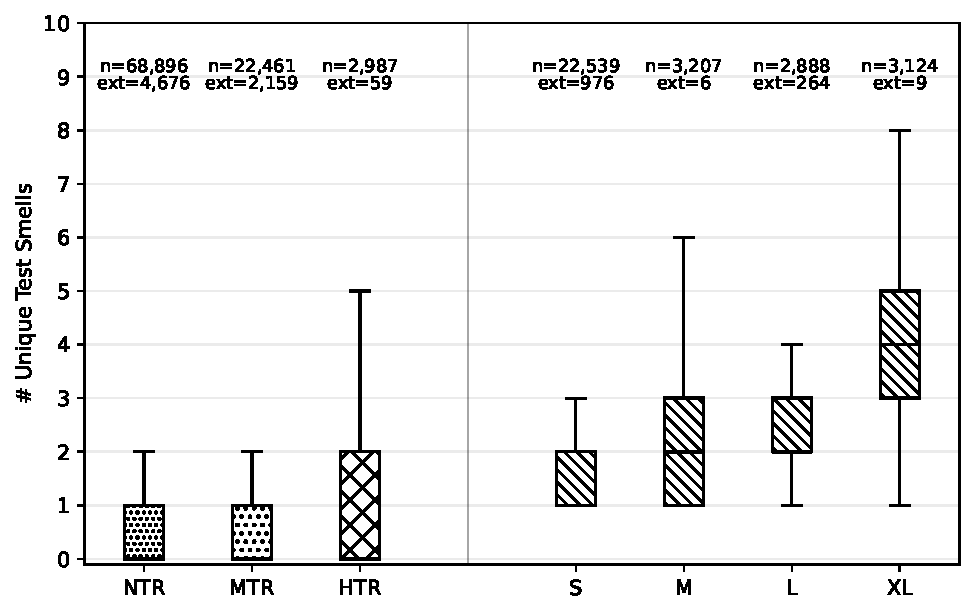
\includegraphics[width=\textwidth]{figure/t2p-test-smell-boxplot--historyFinder--omc--nc--jnose--ch_diff.pdf}
%     \caption{Distribution of the number of unique initial test smells per test method, summarized independently by revision group (NTR and HTR) and by LOC group (S, M, L, and XL). Each box is annotated with the number of methods ($n$) and the number of extreme points outside the boxplot whiskers.}
%     \label{fig:rq4-test-smell-boxplot}
% \end{figure*}

The top part of Table~\ref{tab:rq4-ntr-mtr} shows that, with the exception of a few smell types, such as \emph{Redundant Assertion} and \emph{Lazy Test}, \emph{MTR} methods are more associated with smells than \emph{NTR} methods. For example, 20.1\% of \emph{MTR} methods contain the \emph{Assertion Roulette} smell, compared to 13.5\% of \emph{NTR} methods. The odds ratio (\textbf{OR}) indicates that \emph{MTR} methods are 1.6 times more likely to contain this smell than \emph{NTR} methods. These differences are also statistically significant, as both \textbf{$p_{BH}$} and \textbf{MH $p_{BH}$} are below 0.05.

This trend becomes even more pronounced (bottom part of the table) when comparing \emph{HTR} methods—those revised at least five more times than their corresponding production methods—with \emph{NTR} methods. For most smell types, both the odds ratio and the difference in percent (\textbf{$\Delta$ pp}) increase substantially. In particular, the odds ratios for the \emph{Verbose Test} and \emph{Sleepy Test} smells indicate that these smells are more than six times as likely to occur in \emph{HTR} methods as in \emph{NTR} methods. Overall, Table~\ref{tab:rq4-ntr-mtr} suggests that test methods that evolve more frequently than their corresponding production methods tend to contain more test smells than less change-prone methods.

The potential confounding effect of method size was also examined when interpreting the relationship between test smells and method evolution. Prior studies have shown that many code metrics and smells lose their predictive power for software quality and maintainability once size is controlled for, as size is often strongly correlated with these metrics~\cite{Emam:2001,Gil:2017,TSE:2013}. For this analysis, noise was minimized by excluding smell types that did not exhibit a consistent statistically significant difference in Table~\ref{tab:rq4-ntr-mtr}. Specifically, \emph{Unknown Test}, \emph{Print Statement}, \emph{Redundant Assertion}, \emph{Lazy Test}, \emph{Empty Test}, and \emph{Ignored Test} were excluded. Using the remaining 11 smell types, Kendall's $\tau$ correlation coefficient was computed between size and the number of test smells per method. The resulting coefficient of 0.28 suggests that method size alone does not explain the observed relationship between test smells and method evolution. This apparent discrepancy with previous studies~\cite{Emam:2001,Gil:2017,TSE:2013} is unsurprising, as those studies primarily reported strong correlations between size and software metrics at the class or file level. In contrast, subsequent work has shown that such correlations are considerably weaker at the method level~\cite{Landman:2014,chowdhury:2022}, which is the granularity of this analysis.

To further investigate the impact of method size, following the methodology of Spadini \textit{et al.}~\cite{Spadini:2018}, test methods were categorized into three size groups: small ($size < 30$), medium ($30 \leq size \leq 60$), and large ($size > 60$). Figure~\ref{fig:size} presents the results of this size-stratified analysis. Consistent with the earlier findings, both the difference in percent (\textbf{$\Delta$ pp}) and the odds ratio are larger when comparing \emph{HTR} methods with \emph{NTR} methods than when comparing \emph{MTR} methods with \emph{NTR} methods. More importantly, the association between test smells and method evolution is strongest for small methods: both the percent difference and the odds ratios are considerably larger for small methods than for medium or large methods. This observation contradicts earlier findings~\cite{Spadini:2018} that test smells in large methods are more harmful than smells in smaller methods.


% that test smells present at
% method introduction are more common among HTR methods than among NTR methods.
% The overall difference is substantial: at least one smell is present in
% 49.6\% of HTR methods and 28.8\% of NTR methods. The individual-smell results
% show that this pattern is not uniform across all smell types. Instead, the
% strongest and most stable associations are concentrated in a smaller set of
% smells. Assertion Roulette shows the largest gap, followed by Verbose Test and
% Magic Number Test; Exception Handling and Duplicate Assert also show clear
% increases for HTR methods.

% The project-stratified sensitivity analysis generally supports the main pooled
% results for the strongest smells, indicating that these associations are not
% explained only by differences among projects. However, Eager Test and Lazy Test
% are significant in the pooled analysis but weaken after project adjustment.
% This suggests that these two smell--revision associations are more
% project-dependent and should be interpreted more cautiously.

% Figure~\ref{fig:rq4-test-smell-boxplot} complements the prevalence analysis by
% showing the revision-count distributions of NTR and HTR methods within each
% initial smell category. Because HTR is defined using revision counts, the
% between-group separation is expected; the more informative pattern is which
% smell categories are associated with higher revision counts within the groups.
% Resource Optimism, Mystery Guest, Conditional Test Logic, Print Statement, and
% Exception Handling are among the categories with the highest median revision
% counts in both NTR and HTR. For these smells, the median NTR revision count is
% around two to three revisions, while the corresponding HTR medians are roughly
% nineteen to twenty-two revisions.
% \footnotetext{\href{https://github.com/SQMLab/method-co-evolution/blob/main/data/rqs/rq4/test-smell-difference.pdf}{/data/rqs/rq4/test-smell-difference.pdf}}
\begin{framed}
\noindent\textbf{\underline{RQ4 summary}:}
Smells are more associated with test methods that evolve more than their corresponding production methods. This association becomes even stronger for test methods that are revised at least five more times than their production methods. Furthermore, smells in small test methods show more predictive power than smells in large methods, contradicting earlier findings.
\end{framed}

% RQ4 uses the NTR, MTR, and HTR revision groups defined in RQ3.  The primary
% inferential comparison contrasts NTR and HTR methods because these groups
% separate tests whose revisions do not exceed production revisions from tests
% that accumulate substantially more revisions than their linked production
% methods.  We additionally show the MTR-minus-NTR prevalence difference in the
% effect plot as context for the intermediate revision-prone group, while keeping
% the association table focused on the clearest excess-maintenance contrast.

%  because our unit of analysis
% is the unique test method rather than the test-to-production link. Therefore,
% we omit test methods with conflicting group assignments. Because not all
% projects consistently follow naming conventions when naming test methods after
% their corresponding production methods, the linked-pair strategy identifies
% only a small number of test-production links in some projects.


% For each test method, we identify its introduction commit from the method
% history generated by HistoryFinder. The introduction commit is the earliest
% commit in which the test method appears in the repository. We analyze this
% initial version so that smells are measured before the later revisions used to
% classify recurrent revision-proneness, avoiding the risk of counting smells
% introduced during subsequent maintenance.
